\chapter{Implementierung}
\label{cha:Implementierung}
Zu Prüfungen des Konzepts wurde für die Firma BMD ein Prototyp implementiert. 
Dieser soll zeigen, dass es mit der genannten strukturellen Vorgehensweise möglich ist, ohne großen Wartungsaufwand Schemadateien zu generieren.


\section{Allgemein}
Die Implementierung des Schemagenerators wurde mit Delphi realisiert. Dies wurde von \BMD vorgegeben.
Als Basis für die Umsetzung wurden betriebsinterne Funktionen zum Schreiben von XML-Dokumenten verwendet. 
Diese werden im Unternehmen bereits seit mehreren Jahren verwendet und ausreichend getestet.
Ziel war es hier eine Mischung von einer generischen Umsetzung und kundenspezifischer Lösung zu finden. 
Deswegen wurden explizite Funktionen eingebaut, um Sonderfälle behandeln zu können. Diese können jederzeit erweitert werden.


\begin{figure}
    \centering
    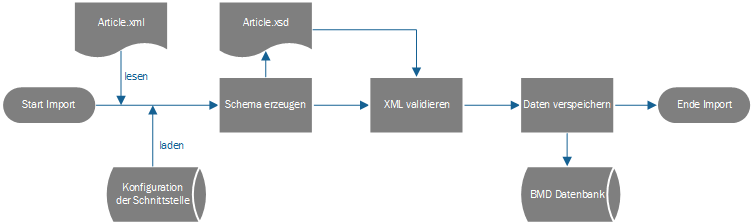
\includegraphics[width=.95\textwidth]{images/Ablaufdiagramm.png}
    \caption{Fertiger Ablauf bei BMD}
    \label{fig:Ablauf}
\end{figure}

Der Prototyp soll direkt in den bestehenden Ablauf bei \BMD integriert werden. Wie man in Abbildung \ref{fig:Ablauf} erkennt, erfolgt die Erstellung der Validierungsdatei, nach dem Lesen der Schnittstellenbeschreibung. Mithilfe der erzeugten Datei (\emph{Article.xsd}), soll nun die zu importierende Datei (\emph{Article.xml}) validiert werden. Ist die Validierung erfolgreich, werden die Daten verarbeitet und in der Datenbank von BMD persistiert.

Die Verarbeitung der XML-Dateien erfolgt bei BMD in der Klasse \emph{TBMDMDPpsTcpXML}. Wie man in Abbildung \ref{fig:Klassenaufbau} erkennt, besitzt diese nun eine Instanz des Validierunsgenerator (\emph{TBMDMDPpsXmlValidationGenerator}), die genutzt wird um das XML Schema zu erzeugen. Die Nomenklatur der Klassen wurde hier von BMD vorgegeben, um den internen Entwicklungsrichtlinien zu entsprechen.

\begin{figure}
    \centering
    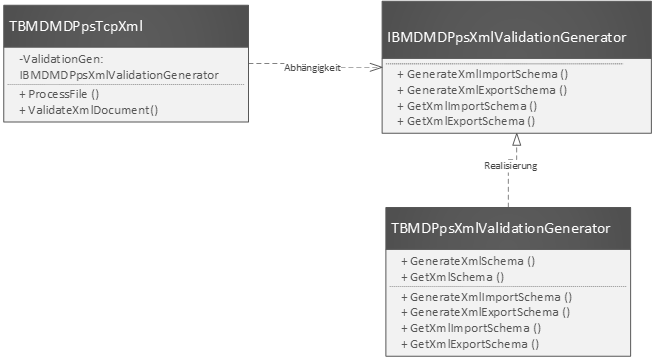
\includegraphics[width=.95\textwidth]{images/KlassenUML_black.png}
    \caption{Klassen-Aufbau}
    \label{fig:Klassenaufbau}
\end{figure}

 
\begin{program}
\caption{Erstellung des Schemas (Ausschnitt)}
 \label{fig:Schemas}
\lstset{language=Pascal, 
        basicstyle=\tiny\ttfamily, 
        numbers=left,
        numberstyle=\tiny, 
        stepnumber=5, 
        firstnumber=0,
        showstringspaces=false}
\lstinputlisting {images/Schema.pas}
\end{program}

\section{XML Schema}
Die Generierung des Schemas kann über zwei Arten erfolgen. 
Entweder wird das Schema nur im Programmspeicher der Anwendung angelegt und zur Validierung im System verwendet, oder das Schema wird auf einem definierten Speicherort abgelegt, siehe Codeauschnitt \ref{fig:Schemas}.

\begin{program}
\caption{Erstellung eines komplexen Datentypen}
 \label{fig:SchemaF}
\lstset{language=Pascal, 
        basicstyle=\tiny\ttfamily, 
        numbers=left,
        numberstyle=\tiny, 
        stepnumber=5, 
        firstnumber=0,
        showstringspaces=false}
\lstinputlisting {images/Schema2.pas}
\end{program}

Das Schema besteht im Detail aus zumindest einem Wurzel-Element in dem alle zulässigen Typen definiert werden können. Diese Art des Aufbaus wurde von BMD vorgegeben, da alle Schnittstellen diesen Aufbau befolgen müssen. Die definierten Typen werden über \emph{complexType}-Elemente abgebildet. Da diese wiederum weitere Typen enthalten können, kann sich diese Methode rekursiv aufrufen (siehe Codeauschnitt \ref{fig:SchemaF}).

 
\begin{program}
\caption{Behandlung von Spezialfällen (Auszug)}
 \label{fig:SchemaE}
\lstset{language=Pascal, 
        basicstyle=\tiny\ttfamily, 
        numbers=left,
        numberstyle=\tiny, 
        stepnumber=5, 
        firstnumber=0,
        showstringspaces=false}
\lstinputlisting {images/Schema3.pas}
\end{program}

Danach können noch etwaige Spezialfälle hinzugefügt werden. Diese sind bereits von bestehenden Schnittstellen vorgegeben und müssen auch in Zukunft gewartet und erweitert werden können (siehe Codeauschnitt \ref{fig:SchemaE}).
 
\section{XML Schematron}
Das Schematron besteht aus fix definierten Regeln, die immer kontextspezifisch sind. 
Deswegen müssen die Regeln für jede Schnittstelle eigens implementiert werden.
Bei der Erstellung des XML Schemas wird aufgrund von fix definierten Kennzahlen ermittelt, ob für diese Schnittstelle ein Schematron umgesetzt wurde und angefügt werden soll (siehe dazu Codeauschnitt \ref{fig:Schematron}).

\begin{program}
\caption{Erstellung des Schematron.}
\label{fig:Schematron}
\lstset{language=Pascal, 
        basicstyle=\tiny\ttfamily, 
        numbers=left,
        numberstyle=\tiny, 
        stepnumber=5, 
        firstnumber=0,
        showstringspaces=false}
\lstinputlisting {images/Schematron.pas}
\end{program}

Wenn für diese Schnittstelle eine oder mehrere Regeln definiert wurden, so wird mittels der \emph{AddPattern}-Funktion, siehe Codeauschnitt \ref{fig:Schematron2} und der \emph{AddRule}-Funktion, siehe Codeauschnitt \ref{fig:Schematron3}, die notwendigen Annotationen eingefügt. Die Regeln werden hier von BMD definiert und müssen händisch im Code hinterlegt werden.

\begin{program}
\caption{Erstellung eines Pattern.}
\label{fig:Schematron2}
\lstset{language=Pascal, 
        basicstyle=\tiny\ttfamily, 
        numbers=left,
        numberstyle=\tiny, 
        stepnumber=5, 
        firstnumber=0,
        showstringspaces=false}
\lstinputlisting {images/Schematron2.pas}
\end{program}

\begin{program}
\caption{Erstellung einer Regel.}
\label{fig:Schematron3}
\lstset{language=Pascal, 
        basicstyle=\tiny\ttfamily, 
        numbers=left,
        numberstyle=\tiny, 
        stepnumber=5, 
        firstnumber=0,
        showstringspaces=false}
\lstinputlisting {images/Schematron3.pas}
\end{program}


\section{Validierung im System}
In Codeauschnitt \ref{fig:ValidationExp} erfolgt die Validierung der Dokumente im System. 
Dies muss am Beginn des Ablaufes stattfinden, da bei einer negativen Validierung ein weiteres Behandeln des Dokuments nicht mehr notwendig und sinnvoll ist. 
Für die Überprüfung des Schemas mit dem XML-Dokument wird das \emph{IXMLDOMDocument2}-Interface verwendet.
Dies ist eine Komponente von Microsoft, die nach Delphi portiert wurde.

\begin{program}
\caption{Validierung im System mit Schematron}
\label{fig:ValidationExp}
\lstset{language=Pascal, 
        basicstyle=\tiny\ttfamily, 
        numbers=left,
        numberstyle=\tiny, 
        stepnumber=5, 
        firstnumber=0,
        showstringspaces=false}
\lstinputlisting {images/validation.pas}
\end{program}

Das Ergebnis der Validierung und etwaige aufgetretene Probleme müssen dem Benutzer mitgeteilt werden können.
Deswegen wurden Schnittstellen für die Kommunikation implementiert, mit denen es möglich ist, Meldungen an den Aufrufer zu liefern (siehe dazu Codeauschnitt \ref{fig:Communication}).

\begin{program}
\caption{Kommunikation von Meldungen und Ergebnissen}
\label{fig:Communication}
\lstset{language=Pascal, 
        basicstyle=\tiny\ttfamily, 
        numbers=left,
        numberstyle=\tiny, 
        stepnumber=5, 
        firstnumber=0,
        showstringspaces=false}
\lstinputlisting {images/Communication.pas}
\end{program}